\def\tutdate{07.02.2018}

\documentclass{beamer}
\usepackage{../templates/beamerthemekit}
%\usepackage{enumitem}

\usepackage[utf8]{inputenc}
\usepackage[T1]{fontenc}
\usepackage[ngerman]{babel}
\usepackage{listings}
\usepackage{hyperref}
\usepackage{graphicx}

\usepackage{amsmath}
\usepackage{amsthm}
\usepackage{amssymb}
\usepackage{polynom}

%\usepackage{ifthen}
%\usepackage{adjustbox} % for \adjincludegraphics

%\usepackage{tikz}
\usepackage{listings}

%\usepackage[]{algorithm2e}

%\usepackage{colortbl}
\usepackage{verbatim}
%\usepackage{alltt}
%\usepackage{changes}

%\usepackage{pdfpages}
%\usepackage{tabularx}

%\usepackage{euler}


\newcommand{\markBlue}[1]{\textcolor{kit-blue100}{#1}}
\newcommand{\markGreen}[1]{\textcolor{kit-green100}{#1}}
\newcommand{\vertspace}{\vspace{.2cm}}

%\newcommand{\#}{\markBlue{#1}}

%\newcommand{\pitem}{\pause\item}
\newcommand{\p}{\pause}

% -- MATH MACROS
\newcommand{\thistheoremname}{}
\newcommand{\G}{\mathbb{Z}}
\newcommand{\B}{\mathbb{B}}
\newcommand{\R}{\mathbb{R}}
\newcommand{\N}{\mathbb{N}}
\newcommand{\Q}{\mathbb{Q}}
\newcommand{\C}{\mathbb{C}}
\newcommand{\Z}{\mathbb{Z}}
\newcommand{\F}{\mathbb{F}}
\newcommand{\mi}{\mathrm{i}}
\renewcommand{\epsilon}{\varepsilon}
\newcommand{\okalk}{\mathscr{O}}


\newenvironment<>{taskblock}[1]{%
	\setbeamercolor{block title}{fg=kit-orange15,bg=kit-orange100}
	\setbeamercolor{block body}{fg=black,bg=kit-orange30}%
	\begin{block}#2{#1}}{\end{block}}

\setbeamertemplate{enumerate items}[default]

% Aussagenlogik Symbole
\newcommand{\W}{w}
\renewcommand{\F}{f}

% Kodierung
\newcommand{\frepr}{\textbf{repr}}
\newcommand{\fRepr}{\textbf{Repr}}
\newcommand{\fZkpl}{\textbf{Zkpl}}
\newcommand{\fbin}{\textbf{bin}}
\newcommand{\fdiv}{\textbf{ div }}
\newcommand{\fmod}{\textbf{ mod }}

% Speicherabbild
\newenvironment{memory}{\begin{tabular}{r | l}Adresse&Wert\\\hline\hline}{\end{tabular}}
\newcommand{\memrow}[2]{#1 & #2 \\\hline}

% Praedikatenlogik
\newcommand{\objequiv}{\stackrel{\cdot}{=}}
\newcommand{\pval}{val_{D,I,\beta}}

% Neue Befehle
\newcommand{\ip}{\pause} % inline pause, für mitten im satz
\newcommand{\pitem}{\pause\item} % für aufzählungen
\newcommand{\bp}{\pause} % block pause, für zwischen blöcken
\title[Grundbegriffe der Informatik]{ICPC\\Gruppe 2}
\date{\tutdate}
\subtitle{\tutTitle}
\author{Elias Schaut, Dennis Kobert, Niklas Kniep, Lam Vo, Ilia Bozhinov}

\institute{}

\titleimage{bg}
%\titleimage{bg-advent}

%
\ifthenelse{\equal{\compiletype}{livebeamer}}
	{
		\def\livebeamermode{1}
	}{}

\ifthenelse{\equal{\compiletype}{print}}
	{
		\def\printmode{1}
	}{}

\setbeamercovered{invisible}

%\usepackage[citestyle=authoryear,bibstyle=numeric,hyperref,backend=biber]{biblatex}
%\addbibresource{templates/example.bib}
%\bibhang1em

	
\def\tutTitle{Relationen, Altklausur}
\begin{document}

\selectlanguage{ngerman}

%title page
\begin{frame}
	\titlepage
\end{frame}

\begin{frame}
\section{Relationen}
Schon bekannte Eigenschaften von Relationen: \newline
\begin{itemize}
	\item transitiv ($\forall x, y, z \in M: (x,y) \in R \land (y, z) \in R \rightarrow (x,z) \in R$)
	\item reflexiv ($\forall x \in M: \rightarrow (x,x) \in R$)
	\item symmetrisch ($\forall x, y \in M: (x,y)  \rightarrow (y,x) \in R$)
		\item Äquivalenzrelation ist reflexiv, transitiv und symmetrisch
\end{itemize}
\end{frame}

\begin{frame}

Neue Eigenschaft: \newline
\begin{itemize}
	\item antisymmetrisch ($\forall x, y \in M: (x,y) \in R \land (y, x) \in R \rightarrow x = y$)
	\item Halbordung ist reflexiv, transitiv und antisymmetrisch
\end{itemize}
\end{frame}

\begin{frame}

Welche Eigenschaften sind hier erfüllt? \newline
\begin{itemize}
	\item $\subset$
	\item $<$
	\item $\leq$
	\item Relation R auf $A^*$ mit v R w $\leftrightarrow \exists u: vu=w$
\end{itemize}
\end{frame}

\section{Master-Theorem}
\begin{frame}
	\begin{block}{Auflösung des Mastertheorem}
	\begin{description}
		\item[Fall 1:] Wenn $f \in \okalk(n^{\log_b a -\epsilon})$ für ein
		$\epsilon>0$ ist, dann ist $T\in \Theta(n^{\log_b a})$.
		\item[Fall 2:] Wenn $f \in \Theta(n^{\log_b a})$ ist, dann ist
		$T\in \Theta(n^{\log_b a}\log n)$.
		\item[Fall 3:] Wenn $f \in \Omega(n^{\log_b a +\epsilon})$ für ein
		$\epsilon>0$ ist, und wenn es eine Konstante $d$ gibt mit $0<d<1$, so
		dass für alle hinreichend großen $n$ gilt $af(n/b)\leq d f$, dann
		ist $T\in \Theta(f)$.
	\end{description}
\end{block}
\end{frame}

\begin{frame}{Pseudocode für Mergesort}
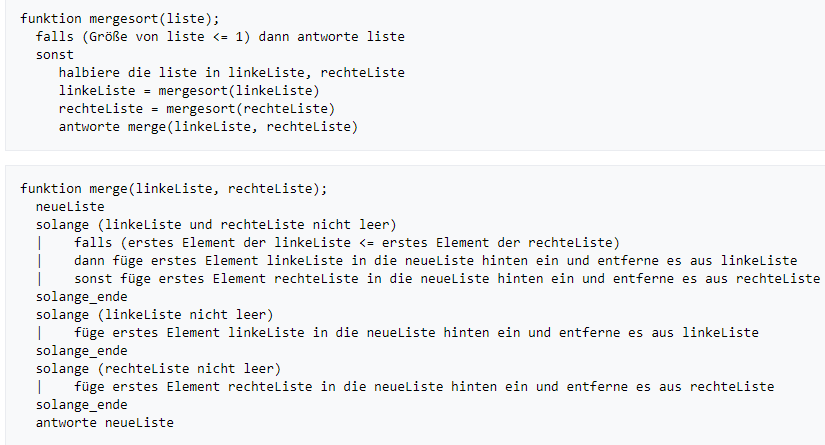
\includegraphics[scale=0.5]{Pseudo.png}
\end{frame}

\begin{frame}
	
\includegraphics[width=\linewidth]{../images/thatsall.png}
\end{frame}


\end{document}